\chapter{نتایج آزمایش‌های تجربی}
\label{chap4:results}
\section{مقدمه}
در این فصل، عملکرد مدل \lr{ProActionCLIP} در زمینه‌ی یادگیری پیوسته‌ی تشخیص حرکت انسان مورد ارزیابی قرار می‌گیرد. هدف از این ارزیابی، بررسی میزان صحت مدل در یادگیری وظایف جدید، ارزیابی میزان فراموشی دانش پیشین و تحلیل بهره‌وری محاسباتی آن از نظر مصرف سخت‌افزار و تعداد پارامترهای قابل‌آموزش است. به منظور ارزیابی جامع، مدل پیشنهادی با روش‌های مطرح در این حوزه مانند \lr{PIVOT} \cite{pivot}و سایر رویکردهای مرجع مقایسه می‌شود. برای این منظور، از مجموعه‌داده‌های نظیر \lr{UCF101} \cite{ucf101} و \lr{HMDB51} \cite{hmdb51} استفاده شده است.

در ادامه‌ی‌ این فصل، ابتدا معیارهای ارزیابی شامل صحت، میزان فراموشی معرفی می‌شوند. سپس، جزئیات مربوط به مجموعه‌های داده، تنظیمات آزمایشی، نتایج و مقایسه ارائه خواهد شد تا ارزیابی مدل پیشنهادی به‌طور کامل و شفاف صورت گیرد. در اخر نیز پیچیدگی محاسباتی بررسی خواهد شد. 
% سخت افزار رو تو همون پیچیدگی محاسباتی بگم. پارامتر. شامل حافظه . بگم رو جی پی یو فلان اموزش دادم. 

\section{معیار‌های ارزیابی}
در یادگیری پیوسته، دو معیار ارزیابی اهمیت دارند. یکی از آن‌ها میانگین صحت وظایف با وجود یادگیری سایر وظایف بوده و دیگری میزان فراموشی مدل پس از یادگیری هر وظیفه است که در ادامه هر یک شرح داده خواهد شد. 
 

\subsection{میانگین صحت}
در یادگیری پیوسته، عملکرد مدل روی تمام وظایف یادگرفته شده تاکنون توسط میانگین صحت ارزیابی می‌گردد. دو نوع صحت $top1$ و $top5$ در این تحقیق بررسی می‌شود. صحت $top1$ بیان‌گر این است که پیش‌بینی‌کننده، از بین احتمالات بدست آمده، برچسب با بیشترین احتمال را انتخاب می‌کند و سپس برابر بودن آن با برچسب واقعی داده‌ی بررسی‌شده، سنجیده می‌‌شود. اما در صحت $top5$، پنج تا برچسب با بیشترین احتمال، انتخاب شده و وجود یا عدم وجود برچسب واقعی در این پنج برچسب بررسی می‌شود. مطابق با \eqref{eq:acc_top_1} و \eqref{eq:acc_top_5}، میانگین صحت در وظیفه‌ی فعلی، برای همین وظیفه و وظایف قبلی، در حالت $top1$ و $top5$ بدست می‌آید. $\text{\lr{ACC}}^{top1}_{i,t}$ نشانگر صحت $top1$ برای وظیفه‌ی $i$ بعد از یادگیری وظیفه‌ی $t$ و $\text{\lr{ACC}}^{top5}_{i,t}$ نشانگر صحت $top5$ برای وظیفه‌ی $i$ بعد از یادگیری وظیفه‌ی $t$ می‌باشد.
\begin{equation}\label{eq:acc_top_1}
	A_{top1}(t) = \frac{1}{t+1} \sum_{i=0}^{t} \text{\lr{ACC}}^{top1}_{i,t}
\end{equation}
\begin{equation}\label{eq:acc_top_5}
	A_{top5}(t) = \frac{1}{t+1} \sum_{i=0}^{t} \text{\lr{ACC}}^{top5}_{i,t}
\end{equation}

\subsection{میزان فراموشی}
در یادگیری پیوسته، مدل باید بتواند وظایف جدید را یاد بگیرد بدون اینکه دانش وظایف قبلی را فراموش کند. اما معمولاً پدیده‌ی فراموشی فاجعه‌آمیز رخ می‌دهد؛ یعنی مدل پس از یادگیری وظایف جدید، صحت آن روی وظایف قدیمی کاهش پیدا می‌کند. معیار فراموشی برای اندازه‌گیری میزان این افت عملکرد تعریف می‌شود و به صورت میانگین کاهش صحت در وظایف قبلی است. بر اساس \eqref{eq:forget_task_i}، فراموشی مدل روی وظیفه‌ی $i$ پس از یادگیری وظیفه‌ی $t$ بدست می‌آید. ماتریس \lr{ACC}، شامل صحت مدل روی هر وظیفه پس از یادگیری همان وظیفه و وظیفه‌های دیگر است. به دنبال آن، $\text{\lr{ACC}}_{i,k}$ نشان‌دهنده‌ی صحت مدل روی وظیفه‌ی $i$ پس از یادگیری وظیفه‌ی $k$ است. به این ترتیب، اختلاف بین بیشترین صحتی که وظیفه‌ی $i$ پس از یادگیری وظایف مختلف بدست آورده و صحتی که پس از وظیفه‌ی $t$ (آخرین وظیفه‌ی یادگرفته شده) بدست آمده، در $f_i(t)$ قرار می‌گیرد. در نهایت فراموشی برای هر وظیفه محاسبه شده و میانگین آن‌ها به عنوان فراموشی مدل پس از یادگیری وظیفه‌ی $t$، در نظر گرفته می‌شود (\eqref{eq:forget_final}). 
\begin{equation}\label{eq:forget_task_i}
	f_i(t) = \max_{k \le t} \text{\lr{ACC}}_{i,k} - \text{\lr{ACC}}_{i,t}
\end{equation}
\begin{equation}\label{eq:forget_final}
	F(t) = \frac{1}{t} \sum_{i=1}^{t} f_i(t) 
\end{equation}

\section{مجموعه‌داده}
در این تحقیق از دو مجموعه‌داده‌ی مرسوم تشخیص حرکت با نام‌های \lr{UCF101}\cite{ucf101} و \lr{HMDB51} \cite{hmdb51} استفاده شده است که در ادامه هریک شرح داده خواهد شد. 

\subsection{مجموعه‌داده‌ی \lr{UCF101}}
مجموعه‌داده‌ی \lr{UCF101} \cite{ucf101} یکی از مجموعه‌داده‌های استاندارد و پرکاربرد در زمینه تشخیص حرکات انسانی در ویدیو است. 
این مجموعه شامل \lr{13{,}320} ویدیو از \lr{101} دسته‌ی مختلف فعالیت انسانی است که طیف وسیعی از حرکات روزمره، ورزشی و تعاملی را پوشش می‌دهد. 
نمونه‌های این مجموعه‌داده از ویدیوهای واقعی و متنوع جمع‌آوری شده‌اند و شامل تغییرات قابل توجه در شرایط نور، پس‌زمینه، زاویه دید و ظاهر اشخاص هستند.
\begin{figure}
	\centering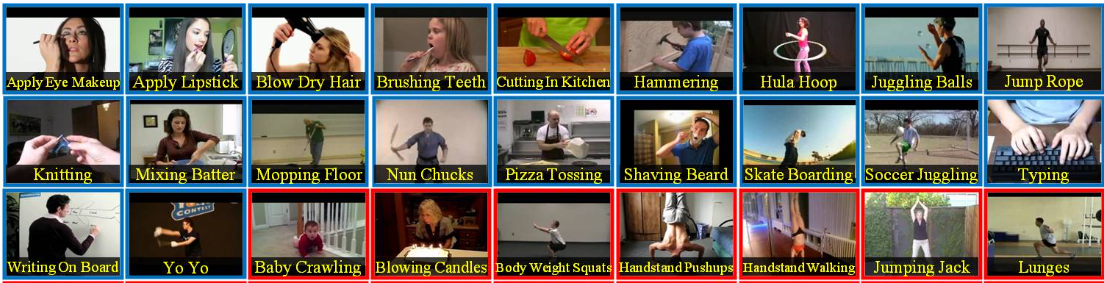
\includegraphics[scale=.5]{Images/Chapter4/ucf101.png}
	\caption[نمونه‌ای از مجموعه‌داده‌ی \lr{UCF101}]{ نمونه‌ای از مجموعه‌داده‌ی \lr{UCF101}\cite{ucf101}.}
	\label{fig.41}
\end{figure}
دسته‌های موجود در \lr{UCF101} به پنج گروه کلی تقسیم می‌شوند:
\begin{enumerate}
	\item \textbf{‌فعالیت‌های ورزشی} 
	\item \textbf{فعالیت‌های تعاملی انسان با اشیا} 
	\item \textbf{فعالیت‌های تعاملی انسان با انسان} 
	\item \textbf{فعالیت‌های بدنی عمومی} 
	\item \textbf{فعالیت‌های نواختن موسیقی} 
\end{enumerate}

ویژگی مهم این مجموعه‌داده، تنوع بالای آن در شرایط تصویربرداری و پیچیدگی حرکات است 
که آن را به یک معیار معتبر برای ارزیابی مدل‌های تشخیص حرکات‌های انسانی و یادگیری پیوسته تبدیل می‌کند. نمونه‌هایی از داده‌های این مجموعه‌داده در \cref{fig.41} قابل مشاهده است. 
‌\subsection{مجموعه‌داده‌ی \lr{HMDB51}}
مجموعه‌داده \lr{HMDB51} \cite{hmdb51} یکی از مجموعه‌داده‌های پرکاربرد در زمینه‌ی تشخیص حرکات انسانی در ویدیو است که برای ارزیابی عملکرد الگوریتم‌های تشخیص حرکت طراحی شده است. 
این مجموعه شامل \lr{6{,}766} ویدیو در \lr{51} دسته‌ی فعالیت انسانی است که هر دسته تقریباً ۱۰۰ نمونه دارد. 
نمونه‌های موجود در \lr{HMDB51} از منابع متنوعی همچون فیلم‌های سینمایی، ویدیو‌های اینترنتی و فیلم‌های خانگی جمع‌آوری شده‌اند 
و طیف وسیعی از حرکات انسانی شامل فعالیت‌های بدنی، تعامل انسان با اشیاء و تعامل انسان با انسان را پوشش می‌دهند. یکی از ویژگی‌های مهم این مجموعه‌داده، تنوع بالا در صحنه، پس‌زمینه، زاویه دوربین و کیفیت ویدیوها است 
که تشخیص حرکات را به یک چالش واقعی تبدیل می‌کند. 
\begin{figure}
	\centering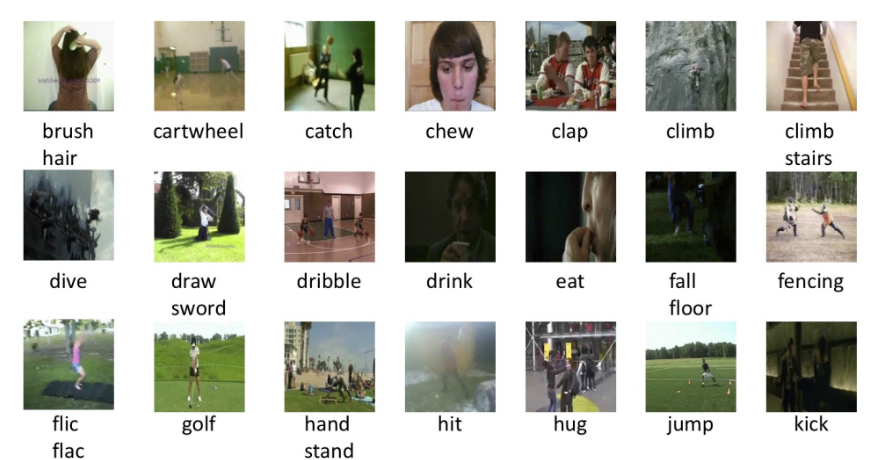
\includegraphics[scale=.6]{Images/Chapter4/HMDB_snapshot1-300x225.png}
	\caption[نمونه‌ای از مجموعه‌داده‌ی \lr{HMDB51}]{ نمونه‌ای از مجموعه‌داده‌ی \lr{HMDB51}\cite{hmdb51}.}
	\label{fig.42}
\end{figure}
به دلیل اندازه متوسط و تنوع مناسب، \lr{HMDB51} به‌طور گسترده برای آموزش و ارزیابی مدل‌های تشخیص حرکات و یادگیری پیوسته مورد استفاده قرار می‌گیرد. فعالیت‌های موجود در \lr{HMDB51} را می‌توان در پنج گروه کلی دسته‌بندی کرد:
\begin{enumerate}
	\item \textbf{فعالیت‌های عمومی صورت}
	\item \textbf{فعالیت‌های صورت همراه با تعامل با اشیا} 
	\item \textbf{حرکات عمومی بدن} 
	\item \textbf{حرکات بدن همراه با تعامل با اشیا} 
	\item \textbf{حرکات بدن در تعامل انسان با انسان} 
\end{enumerate}
نمونه‌ای از این داده‌ها در \cref{fig.42} قابل مشاهده است.
\section{تنظیمات آزمایش}
آزمایش‌ها بر روی دو مجموعه‌داده‌ی \lr{HMDB51}\cite{hmdb51} و \lr{UCF101}\cite{ucf101} به صورت جداگانه اجرا شده و در هر دو حالت، مدل پایه‌ی مورد استفاده، \lr{Open-VCLIP} \cite{open-vclip} می‌باشد که در فرآیند آموزش از وزن‌های پیش‌آموخته‌ی \lr{CLIP} \cite{clip} (نسخه‌ی \lr{ViT-B/16}) بهره برده است. آموزش با نرخ اولیه‌ی یادگیری $3.33 \times 10^{-6}$ (مقدار معین شده در تنظیمات \lr{Open-VCLIP}) تست گردید اما به علت یادگیری آهسته و دریافت نتیجه‌ی نامطلوب، نرخ اولیه‌ی یادگیری، بعد از آزمایش‌های مختلف، با مقدار $1.5 \times 10^{-3}$ برای مجموعه‌داده‌ی \lr{UCF101} و $1.5 \times 10^{-2}$ برای مجموعه‌داده‌ی \lr{HMDB51} مورد استفاده قرار گرفت. مجموعه‌داده‌ها به نسبت‌های $60\%$ برای آموزش، $30\%$ برای آزمون و $10\%$ برای اعتبارسنجی تقسیم شدند. تعداد وظیفه‌‌ برای هر اجرا، $10$ در نظر گرفته شد و تعداد دسته‌‌ در هر وظیفه‌، برابر با تعداد کل ‌دسته‌‌های مجموعه8‌داده تقسیم بر تعداد کل وظایف خواهد بود. تنظیمات مربوط به پرامپت، شامل طول هر پرامپت، مقدار بیشینه‌ تعداد پرامپت انتخابی در هر اجرا، به ترتیب 5 (طبق مقداردهی \lr{L2P} \cite{l2p})و 2 در نظر گرفته شده است.  طول استخر پرامپت متناسب با سناریوی استفاده شده، متفاوت خواهد بود. سایر تنظیمات، مانند تنظیمات معرفی شده در \lr{Open-VCLIP}، در نظر گرفته شده‌اند. در ادامه تنظیمات اجرا برای هر دو مجموعه‌داده‌ی مذکور بررسی خواهند شد. سخت افزار استفاده شده در این تحقیق، \lr{GPU L40S} با $48$ گیگابایت حافظه‌ی رم می‌باشد. 
\subsection{آزمایش با مجموعه‌داده‌ی \lr{UCF101}}
در این آزمایش ابتدا تعداد $5$ ایپاک برای هر وظیفه در نظر گرفته شد و پس از بررسی نمودار صحت بر حسب ایپاک طی شده، مشاهده شد که صحت وظایف پس از سه ایپاک چه در اعتبارسنجی و چه در آموزش ثابت می‌شوند. بنابراین ایپاک نهایی برای این مجموعه‌داده، $3$ در نظر گرفته شد. آزمایش این مجموعه‌داده در سه سناریو بررسی شد که در ادامه توضیح داده خواهد شد: 
\begin{enumerate}
	\item \textbf{استخر ثابت با جریمه‌ی وزن‌های پیشین:} 
	دراین حالت طول استخر پرامپت ثابت خواهد بود که در این آزمایش، به اندازه‌ی $202$ مقداردهی شده است. تعداد تکرار انتخاب هر پرامپت در یادگیری پیوسته، ذخیره می‌شود و هنگام انتخاب پرامپت در وظیفه‌ی جدید، متناسب با تعداد تکرار هر پرامپت، جریمه‌ای در نظر گرفته می‌شود. بنابراین احتمال انتخاب پرامپت‌های پیشین، تا حدودی کاهش می‌یابد(الگو گرفته از روش اضافه‌ی ذکر شده در \lr{L2P} \cite{l2p}).  
	\item \textbf{استخر پویا با مقداردهی تصادفی:}
	در این حالت طول استخر پرامپت اولیه به اندازه‌ی $20$ در نظر گرفته شده است. هر وظیفه‌‌ که اضافه می‌شود، به طول استخر $20$ واحد اضافه می‌شود. نکته‌ی حائز اهمیت در سناریوی فعلی و بعدی، این است که پرامپت‌های استفاده شده در وظایف قبلی، هنگام یادگیری وظیفه‌ی جدید، منجمد شده و صرفا قابلیت انتخاب شدن، دارند و تغییری نخواهند کرد. 
	\item \textbf{استخر پویا با مقداردهی مبتنی بر کدگذار متن \lr{CLIP}:}
	در این حالت، تمام تنظیمات مدل مشابه سناریوی قبلی است و تنها تفاوت، در نحوه‌ی مقداردهی اولیه‌ی کلیدهای استخر پرامپت است. در ابتدا، به ازای هر دسته‌ در هر وظیفه، به تعداد از پیش‌تعیین‌شده کلید، مقداردهی اولیه می‌شود؛ به این صورت که برچسب هر دسته به همراه عبارت‌های معنادار ثابت، از کدگذار متن مدل \lr{CLIP} عبور کرده و ویژگی‌های استخراج‌شده در کلیدها قرار می‌گیرند. به عنوان مثال اگر برچسب یک ویدیو، \lr{jumping person}  باشد، عبارتی که وارد کدگذار می‌شود برابر با \lr{\texttt{"a video of jumping person."}} خواهد بود. در این سناریو، مقادیر اولیه‌ی کلیدها معنادار بوده و نتایج نشان داده اند که تاثیر مثبتی در انتخاب درست پرامپت‌ها داشته‌اند. در آزمایش اولیه، تعداد کلیدهای مقداردهی اولیه برای هر دسته از هر وظیفه‌، برابر با $2$ در نظر گرفته شد. در حالت نهایی تست‌شده، برای بهبود انتخاب پرامپت‌ها، این تعداد به $5$ کلید برای هر دسته افزایش یافت که این تغییر باعث شد که فضای انتخاب پرامپت‌ها غنی‌تر شود و مدل در انتخاب پرامپت‌های مناسب عملکرد بهتری داشته باشد.
\end{enumerate}

\subsection{آزمایش با مجموعه‌داده‌ی \lr{HMDB51}}
یش ابتدا تعداد $5$ ایپاک برای هر وظیفه در نظر گرفته شد و پس از بررسی نمودار صحت بر حسب ایپاک طی شده، مشاهده شد که یادگیری به خوبی صورت نگرفته است. بنابراین پس از افزایش ایپاک‌ها در طی آزمایش، ایپاک نهایی برای این مجموعه‌داده، $7$ در نظر گرفته شد. مانند مجموعه‌داده‌ی پیشین، آزمایش این مجموعه‌داده نیز در سه سناریو بررسی شد که در ادامه توضیح داده خواهد شد: 
\begin{enumerate}
	\item \textbf{استخر ثابت با جریمه‌ی وزن‌های پیشین:} 
	این سناریو نیز مانند توضیحات ذکر شده در قسمت قبل، اجرا شده است با این تفاوت که طول استخر پرامپت در این جا $102$ در نظر گرفته شده است.   
	\item \textbf{استخر پویا با مقداردهی تصادفی:}
	در این حالت طول استخر پرامپت اولیه ابتدا به اندازه‌ی $10$ در نظر گرفته شد و سپس به علت کسب نتیجه‌ی بهتر، به $25$ تغییر داده شد. هر وظیفه‌‌ که اضافه می‌شود، به طول استخر $25$ واحد اضافه می‌شود. نکته‌ی حائز اهمیت در سناریوی فعلی و بعدی، این است که پرامپت‌های استفاده شده در وظایف قبلی، هنگام یادگیری وظیفه‌ی جدید، منجمد شده و صرفا قابلیت انتخاب شدن، دارند و تغییری نخواهند کرد. 
	\item \textbf{استخر پویا با مقداردهی مبتنی بر کدگذار متن \lr{CLIP}:}
	همانند آن‌چه در قسمت مجموعه‌داده‌ی \lr{UCF101} گفته شد، تنظیمات مانند سناریوی پیشین باقی می‌مانند و صرفا مقداردهی اولیه‌ی کلیدها با کدگذار \lr{CLIP} صورت می‌گیرد. در این جا نیز ابتدا تعداد کلیدهای مقداردهی اولیه برای هر دسته از هر وظیفه‌، برابر با $2$ در نظر گرفته شد و در نهایت، این تعداد به $5$ کلید برای هر دسته افزایش یافت. به عبارتی، طول اولیه‌ی استخر پرامپت از $10$ به $25$ تغییر داده شد. 
\end{enumerate}


\section{ارزیابی نتایج}
به‌منظور ارزیابی عملکرد روش 
\lr{ProActionCLIP}
با سایر روش‌های مشابه، ابتدا مدل تنها با داده‌های مربوط به وظیفه‌ی اول آموزش داده می‌شود و سپس وظایف بعدی به‌ترتیب به مدل معرفی و آموزش داده می‌شوند. در این فرآیند، مدل باید ضمن یادگیری اطلاعات مربوط به هر وظیفه‌ی جدید، دانش حاصل از وظایف قبلی را نیز حفظ کند. پس از اتمام یادگیری تمامی ده وظیفه، دو معیار میزان فراموشی و میانگین صحت، برای ارزیابی عملکرد مدل، مورد استفاده قرار می‌گیرد. میانگین صحت، نشان‌دهنده‌ی توانایی مدل در حفظ عملکرد بر روی تمام وظایف است و میزان فراموشی، نشان‌دهنده‌ی کاهش صحت مدل، بر روی وظایف اولیه، پس از یادگیری وظایف جدید می‌باشد. این دو معیار برای مقایسه‌ی دقیق‌تر بین روش پیشنهادی و سایر روش‌های موجود به‌کار گرفته شده‌اند. 
نتایج حاصل از ارزیابی عملکرد روش \lr{ProActionCLIP} و سایر روش‌های منتخب، در جدول
\ref{table:ucf101_results}
آورده شده است. در این جدول علاوه بر میانگین صحت و میزان فراموشی، تعداد پارامترهای آموزش‌پذیر مدل و میزان حافظه‌ برای نگه‌داری نمونه‌های ویدیویی وظایف پیشین نیز مقایسه شده است.
روش‌های مقایسه‌شده شامل \lr{iCaRL}\cite{11}،
 \lr{EWC}\cite{7}،
  \lr{L2P}\cite{l2p}،
 \lr{Pivot}\cite{pivot} و \lr{Open-VCLIP}\cite{open-vclip} می‌باشند. این روش‌ها نماینده‌ی رویکردهای متنوع در حوزه‌ی یادگیری پیوسته هستند. روش‌های \lr{iCaRL}، \lr{EWC} و \lr{L2P} در اصل برای داده‌های تصویری طراحی شده‌اند، اما با استناد به دو مطالعه‌ی پیشین \cite{vclimb,rainbowprompt} که این روش‌ها را بر روی داده‌های ویدیویی مجموعه‌داده‌ی \lr{UCF101} مورد ارزیابی قرار داده‌اند، نتایج مربوط به آن‌ها نیز در
جدول~\ref{table:ucf101_results}
گزارش شده‌اند. در جدول فوق همچنین از مدل \lr{Open-VCLIP} در حالت منجمد استفاده شده است.  در این حالت، وظایف به ترتیب به مدل ارائه شدند تا صحت آن در مواجهه با وظایف جدید اندازه‌گیری شود. برای این مدل در هر مرحله از آزمایش تنها تنها تعداد دسته‌ها نسبت به مرحله قبل افزایش یافته است.
  
 \begin{table}
 	\centering
 	\caption[مقایسه‌ی روش پیشنهادی با سایر روش‌ها]{مقایسه روش \lr{ProActionCLIP} با سایر روش‌های یادگیری پیوسته روی مجموعه‌داده \lr{UCF101} بر اساس  صحت، میزان فراموشی، تعداد پارامترها و حافظه مورد استفاده.}
 	\label{table:ucf101_results}
 	\begin{LTR}
 		\resizebox{0.95\textwidth}{!}{
 			\begin{tabular}{l|c|c|cc}
 				\hline
 				\lr{\textbf{Model}} & \lr{\textbf{Memory usage. Number of Video Instances}} & \lr{\textbf{Params}} & \multicolumn{2}{c}{\lr{\textbf{UCF101}}} \\
 				& & & \lr{\textbf{Accuracy [\%]}} & \lr{\textbf{Forgetting [\%]}} \\
 				\hline
 				\lr{PIVOT} & \lr{1010} & \lr{9M} & \lr{93.36} & \lr{4.47} \\
 				\lr{iCaRL} & \lr{2020} & \lr{0.5M} & \lr{80.97} & \lr{18.11} \\
 				\lr{EWC} & \lr{None} & \lr{0.4} & \lr{9.51} & \lr{98.94} \\
 				\lr{L2P} & \lr{None} & \lr{124K} & \lr{78.35} & \lr{5.46} \\
 				\lr{Open-VCLIP} & \lr{None} & \lr{None} & \lr{79.64} & \lr{-} \\
 				\lr{ProActionCLIP (Ours)}  & \lr{None} & \lr{2M} & \lr{81.07} & \lr{9.44} \\
 				\hline
 			\end{tabular}
 		}
 	\end{LTR}
 \end{table}
 
 در جدول~\ref{table:ucf101_results}، همان‌طور که مشاهده می‌شود مدل پیشنهادی، از لحاظ میانگین صحت و میزان فراموشی، نتایج بهتری نسبت به سایر روش‌های مشابه داشته است. البته روش \lr{PIVOT} در مقایسه با روش پیشنهادی، صحت بیشتر و میزان فراموشی کمتری کسب کرده است. علت این امر، استفاده این روش از حافظه برای ذخیره‌ی داده‌های ویدیویی وظایف پیشین بوده است. علاوه بر حافظه‌ مصرفی، تعداد پارامترهای قابل یادگیری این روش به میزان قابل توجهی نسبت به روش پیشنهادی، بیشتر است. انتظار می‌رود استفاده از حافظه و تعداد پارامترهای قابل یادگیری بیشتر، در افزایش صحت و کاهش میزان فراموشی مدل‌ها موثر باشند. این امر در جدول~\ref{table:ucf101_results} قابل مشاهده است. چنان‌که مدل \lr{Open-VCLIP} به صورت منجمد استفاده شده است و از حافظه و پارامتر قابل‌آموزش بهره نبرده است، صحت کمتری نسبت به \lr{PIVOT} ارائه داده است. با این حال، این مدل علیرغم آنکه برای یادگیری پیوسته طراحی نشده است، نتایج نسبتا خوبی در حالت یادگیری بدون نمونه ارائه داده است. یکی از دلایلی که این روش در معماری 
 \lr{ProActionCLIP}
 به‌کار گرفته شده است، همین موضوع می‌باشد. در مدل \lr{EWC}، از حافظه استفاده نشده است. این مدل برای تصویر آموزش داده شده است و نتایج نامطلوب ارائه شده برای ویدیو، به این علت است که از ویدیو، صرفا تعداد محدودی قاب برای دسته‌بندی انتخاب شده است و از مدل‌های از پیش آموزش دیده مانند \lr{CLIP} نیز استفاده نکرده است. در مدل \lr{iCaRL}، استفاده از حافظه، باعث افزایش صحت شده است اما میزان فراموشی هم‌چنان نسبت به مدل پیشنهادی، بالاتر است. در روش \lr{L2P} با وجود استفاده نکردن از حافظه و آموزش پارامترهای قابل یادگیری کم، توانسته است نتایج خوبی ارائه دهد. این ویژگی‌های مثبت در روش \lr{Open-VCLIP} و \lr{L2P} موجب ارائه‌ی روش 
 \lr{ProActionCLIP}
 گردید که توانسته است نسبت به این دو روش، نتایج بهتری را ارائه دهد.
 
 به منظور ارائه‌ی مقایسه‌ا‌ی دقیق‌تر بین روش پیشنهادی و \lr{Open-VCLIP}، میانگین صحت وظایف در هر گام آموزشی محاسبه گردید که نتایج آن برای مجموعه‌‌داده‌های 
 \lr{UCF101} و
 \lr{HMDB51}
 به ترتیب در نمودارهای \cref{fig.43} و \cref{fig.44} آورده شده است. 
 \begin{figure}
 	\centering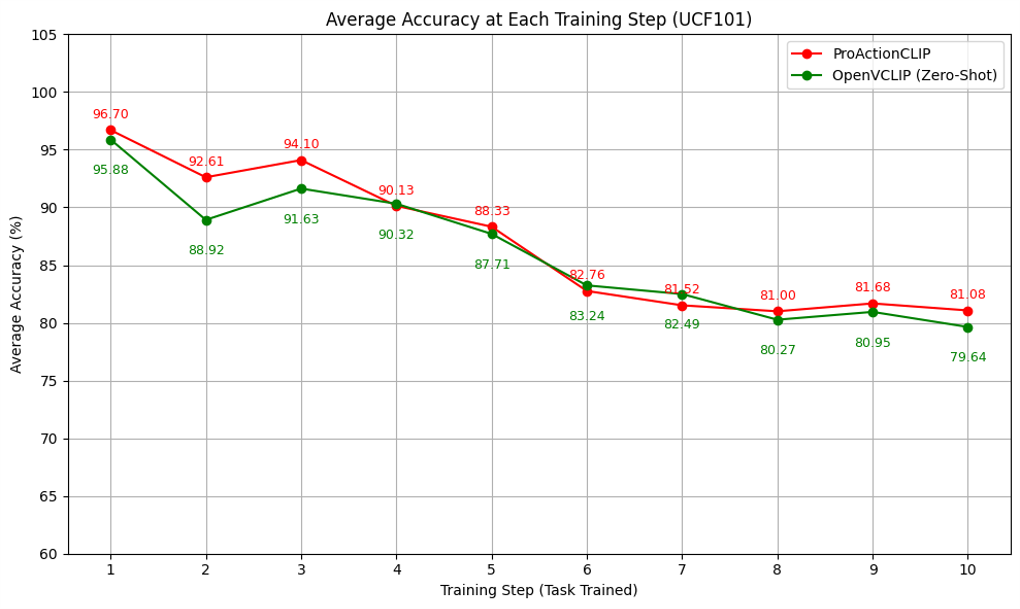
\includegraphics[scale=.6]{Images/Chapter4/ucf101_zeroshot.png}
 	\caption[میانگین صحت وظایف در هر گام آموزشی برای مجموعه‌داده‌ی \lr{UCF101} ]{میانگین صحت وظایف در هر گام آموزشی برای دو روش 
 	 \lr{ProActionCLIP} و
 	\lr{Open-VCLIP}
 	برای مجموعه‌داده‌ی \lr{UCF101}.
 	محور عمودی نشان‌دهنده‌ی میانگین صحت مدل بر وظایف و محور افقی نشان‌دهنده‌ی گام‌های آموزش است. در هر گام آموزشی، یک وظیفه اضافه می‌شود. با افزایش تعداد وظایف و در نتیجه افزایش تعداد دسته‌ها، میانگین صحت کاهش می‌یابد. نمودار قرمزرنگ مربوط به مدل پیشنهادی بوده و نمودار سبزرنگ  مربوط به مدل \lr{Open-VCLIP} ‌‌می‌باشد. 
 	}
 	\label{fig.43}
 \end{figure}
  \begin{figure}
 	\centering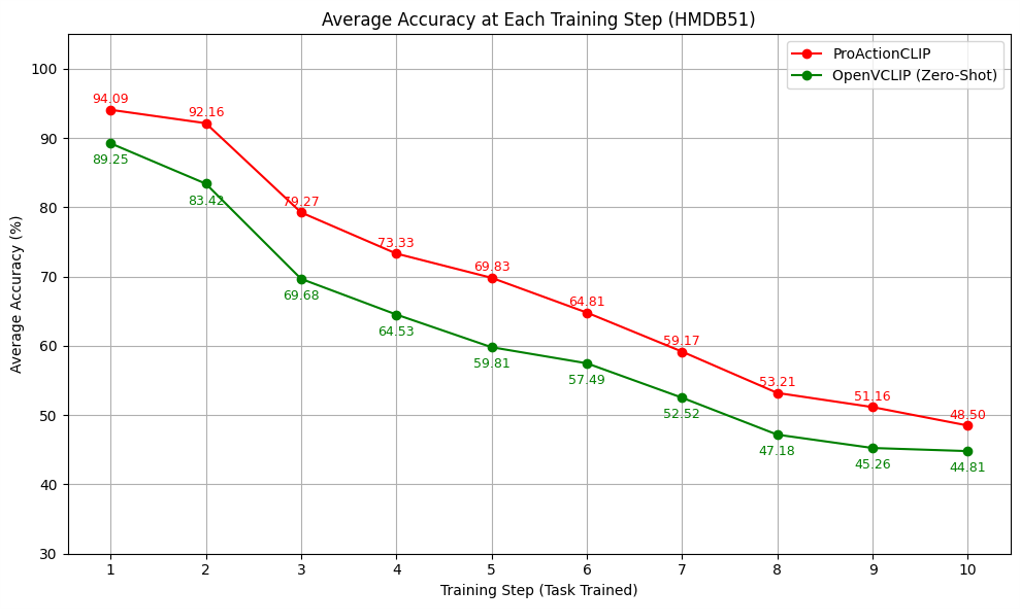
\includegraphics[scale=.6]{Images/Chapter4/hmdb_zeroshot.png}
 	\caption[مجموعه‌داده‌ی \lr{HMDB51}]{ میانگین صحت وظایف در هر گام آموزشی برای دو روش 
 		\lr{ProActionCLIP} و
 		\lr{Open-VCLIP}
 		برای مجموعه‌داده‌ی \lr{HMDB51}  .
 		محور عمودی نشان‌دهنده‌ی میانگین صحت مدل بر وظایف و محور افقی نشان‌دهنده‌ی گام‌های آموزش است. در هر گام آموزشی، یک وظیفه اضافه می‌شود. با افزایش تعداد وظایف و در نتیجه افزایش تعداد دسته‌ها، میانگین صحت کاهش می‌یابد. نمودار قرمزرنگ مربوط به مدل پیشنهادی بوده و نمودار سبزرنگ  مربوط به مدل \lr{Open-VCLIP} ‌‌می‌باشد. 
 		
 		}
 	\label{fig.44}
 \end{figure}
 \begin{comment}
 	.همانطور که مشاهده می‌شود در این نمودارها با افزایش وظایف، صحت میانگین روند نزولی داشته است. علت وقوع این امر آن است که با اضافه شدن وظیفه‌ی جدید، تعداد دسته‌ها افزایش می‌یابد. در واقع در این روش‌ها، با اضافه شدن وظیفه‌ی جدید، ویژگی بدست آمده از داده‌ی ویدیویی باید با تعداد دسته‌ی بیشتری مقایسه شود و احتمال ایجاد خطا در تصمیم‌گیری و کاهش صحت بالا می‌رود. با این حال، همان‌طور که مشاهده می‌شود، مدل پیشنهادی در هر دو مجموعه‌داده بهتر عمل کرده است. ..
 \end{comment}
همان‌طور که مشاهده می‌شود، در این نمودارها با افزایش تعداد وظایف، میانگین صحت روندی نزولی داشته است. یکی از دلایل این امر آن است که با اضافه شدن هر وظیفه‌ی جدید، تعداد دسته‌ها افزایش یافته و ویژگی استخراج‌شده از ویدیو باید با تعداد بیشتری دسته مقایسه شود. این موضوع احتمال بروز خطا در تصمیم‌گیری و کاهش صحت را بالا می‌برد. علاوه بر این، شباهت معنایی برخی برچسب‌ها نیز می‌تواند عامل دیگری برای افت صحت باشد. برای مثال، در مجموعه‌داده‌ی \lr{UCF101} دسته‌هایی مانند
\lr{Playing Guitar}، \lr{Playing Piano}، \lr{Playing Tabla}، \lr{Playing Violin}، \lr{Playing Cello}، \lr{Playing Daf}، \lr{Playing Dhol}، \lr{Playing Flute} و \lr{Playing Sitar}
همگی عبارت مشترک \lr{"Playing"} را در برچسب خود دارند. این شباهت باعث می‌شود که در فرایند کدگذاری متن توسط مدل \lr{CLIP}، نمایش‌های برداری این برچسب‌ها به یکدیگر نزدیک شوند و در نتیجه، کلیدهای پرامپت این دسته‌ها نیز، شباهت بالایی به یکدیگر پیدا کنند. در چنین شرایطی، ممکن است مدل برای یک ویدیوی مرتبط با یکی از این دسته‌ها، به اشتباه پرامپت دسته‌ی مشابه دیگری را انتخاب کند. با این حال، نتایج نشان می‌دهد که مدل پیشنهادی در هر دو مجموعه‌داده عملکرد بهتری در کاهش این افت صحت داشته است.
 \subsection{مطالعات فرسایشی}
به‌منظور بررسی تأثیر مؤلفه‌های مختلف مدل پیشنهادی \lr{ProActionCLIP}، یک مطالعه‌ی فرسایشی\LTRfootnote{Ablation study}
انجام گرفته است. مدل \lr{ProActionCLIP} در این پژوهش به‌عنوان ترکیبی از دو روش \lr{Open-VCLIP} و \lr{L2P} طراحی شده و در دو مجموعه‌داده‌ی معتبر \lr{HMDB51} و \lr{UCF101} مورد ارزیابی قرار گرفته است.
برای تحلیل دقیق‌تر، مطابق با آن‌چه در قسمت تنظیمات آزمایش ذکر شد، عملکرد مدل در سه پیکربندی متفاوت از نظر ساختار و رفتار استخر پرامپت‌ها مورد آزمایش قرار گرفت. این پیکربندی‌ها عبارتند از:

\begin{enumerate}
	\item \textbf{استخر ثابت با جریمه:} طول استخر ثابت نگه داشته شده و با استفاده از سازوکار جریمه، احتمال استفاده‌ی مجدد از پرامپت‌های پرتکرار کاهش می‌یابد.
	
	\item \textbf{استخر پویا با مقداردهی تصادفی:} با ورود هر وظیفه، پرامپت‌های جدید به‌صورت تصادفی اضافه شده و پرامپت‌های قبلی منجمد می‌شوند.
	
	\item \textbf{استخر پویا با مقداردهی معنایی:} مشابه سناریوی قبل، اما مقداردهی اولیه‌ی پرامپت‌ها با استفاده از خروجی کدگذار متن \lr{CLIP}  انجام می‌شود.
\end{enumerate}
نتایج حاصل از این آزمایش‌ها برای مجموعه‌داده‌های \lr{UCF101} و \lr{HMDB51} به ترتیب در 
\cref{fig:ablation_study_ucf101}
و
\cref{fig:ablation_study_hmdb}
آورده شده است که در ادامه هر یک بررسی خواهد شد. مطابق آنچه در \cref{fig:ablation_study_ucf101} مشاهده می‌شود، نتایج روی مجموعه‌داده‌ی 
\lr{UCF101}
نشان می‌دهد که استفاده از مقداردهی اولیه با کدگذار \lr{CLIP} موجب حفظ بهتر صحت در طول گام‌های آموزشی می‌شود و این اثر با افزایش تعداد پرامپت‌های هر دسته از دو به پنج، تقویت می‌گردد. مقایسه‌ی \cref{subfig:Encoder init 5 prompts class dynamic pool} و \cref{subfig:Encoder init 2 prompts class dynamic pool} نشان می‌دهد که افزایش تعداد پرامپت‌ها باعث بهبود عملکرد، به‌ویژه در گام‌های پایانی آموزش و کاهش نرخ افت صحت یا همان فراموشی شده است. در مقابل، در دو پیکربندی با مقداردهی اولیه تصادفی، عملکرد کلی پایین‌تر بوده و افت صحت در طول مراحل آموزش محسوس‌تر است. همچنین مقایسه‌ی \cref{subfig:Random init 2 prompts class dynamic pool} و \cref{subfig:Random init fixed pool} نشان می‌دهد که استفاده از استخر پرامپت پویا در مقداردهی تصادفی نسبت به استخر ثابت، موجب بهبود نسبی حفظ صحت می‌شود. این نتایج بیانگر آن است که هم نوع مقداردهی اولیه و هم طراحی استخر پرامپت نقش کلیدی در کاهش فراموشی و بهبود پایداری مدل در یادگیری وظایف پیوسته دارند. با توجه به اینکه نتایج سناریوی آخر در مجموعه‌داده‌ی \lr{UCF101} عملکرد بهتری داشت، همان سناریو برای مجموعه‌داده‌ی \lr{HMDB51} نیز مورد ارزیابی قرار گرفت و نتایج آن در \cref{fig:ablation_study_hmdb} ارائه شده است. همان‌طور که مشاهده می‌شود، هر دو پیکربندی از مقداردهی اولیه با کدگذار \lr{CLIP} استفاده می‌کنند و تفاوت اصلی آن‌ها در تعداد پرامپت‌های هر دسته است. مقایسه‌ی \cref{subfig:Encoder init 5 prompts class dynamic pool hmdb} و \cref{subfig:Encoder init 2 prompts class dynamic pool hmdb} نشان می‌دهد که افزایش تعداد پرامپت‌ها از دو به پنج موجب بهبود عملکرد مدل، به‌ویژه در مراحل پایانی آموزش، و کاهش نرخ افت صحت یا همان فراموشی شده است. این نتایج نشان می‌دهد که حتی در شرایطی که نوع مقداردهی اولیه ثابت باشد، افزایش تعداد پرامپت‌های هر دسته می‌تواند نقش مؤثری در حفظ دانش و پایداری مدل در طول یادگیری وظایف پیوسته ایفا کند.
\begin{figure}
	\centering
	\subfloat[استخر پویا\lr{CLIP init – 5/class – }]{
		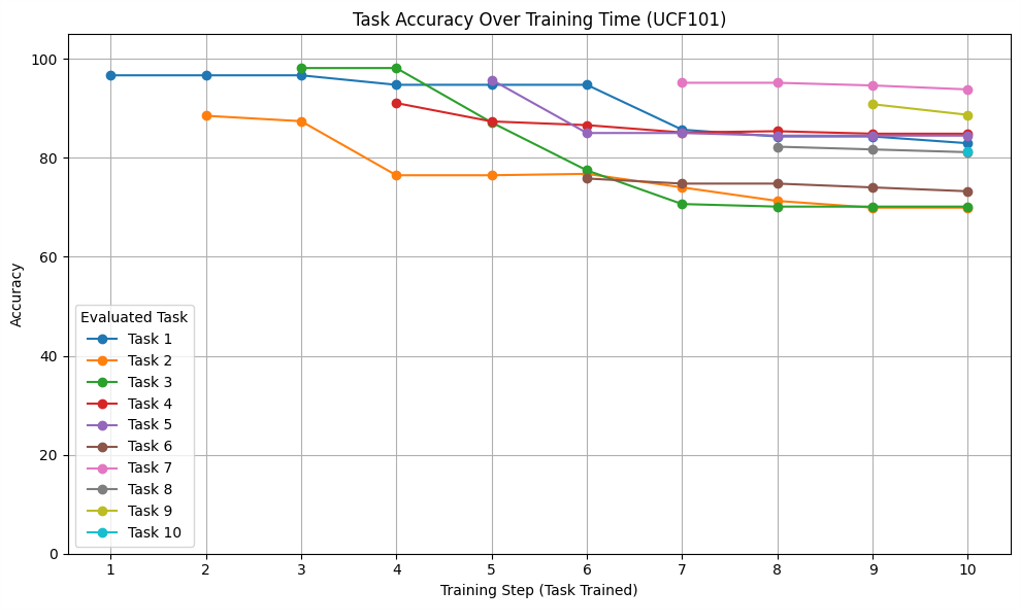
\includegraphics[width=0.45\textwidth]{Images/Chapter4/Encoder init 5 prompts class dynamic pool.png}
		\label{subfig:Encoder init 5 prompts class dynamic pool}
	}
	\quad
	\subfloat[استخر پویا\lr{CLIP init – 2/class – }]{
		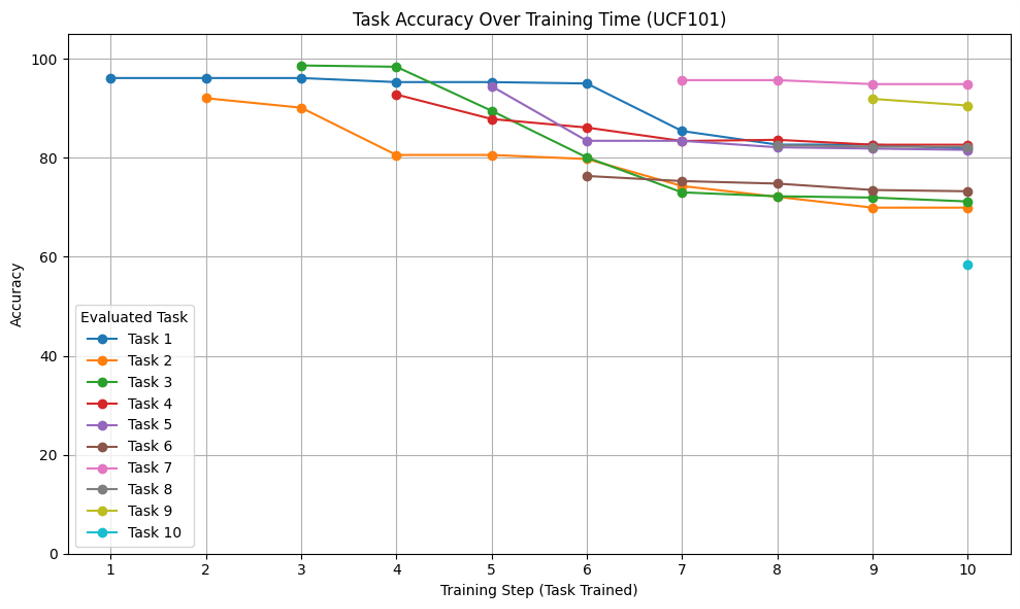
\includegraphics[width=0.45\textwidth]{Images/Chapter4/Encoder init 2 prompts class dynamic pool.png}
		\label{subfig:Encoder init 2 prompts class dynamic pool}
	}
	\\
	\subfloat[استخر پویا\lr{Random init – 2/class – }]{
		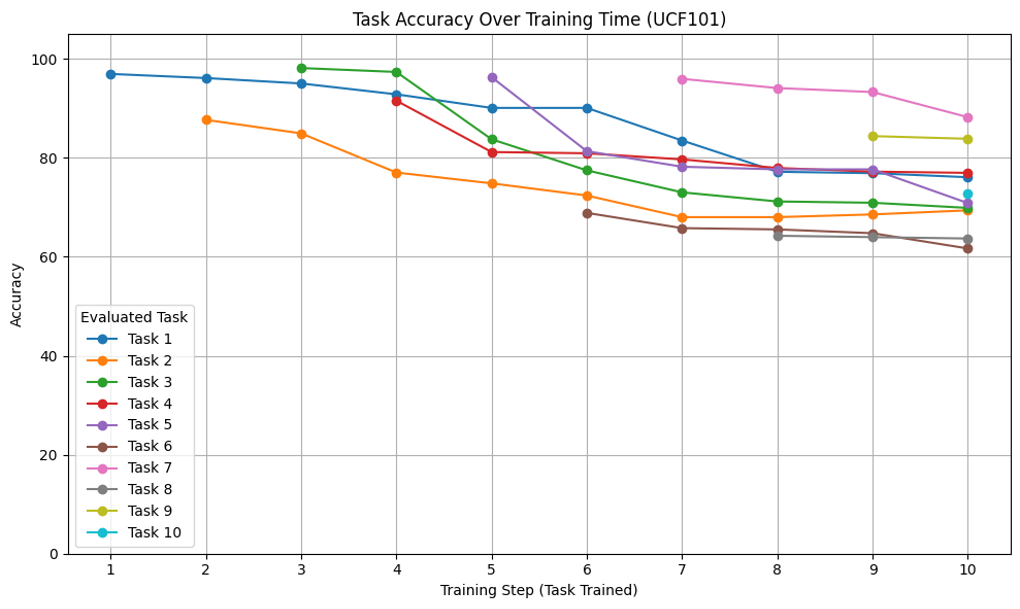
\includegraphics[width=0.45\textwidth]{Images/Chapter4/Random init 2 prompts class dynamic pool.png}
		\label{subfig:Random init 2 prompts class dynamic pool}
	}
	\quad
	\subfloat[استخر ثابت\lr{Random init – }]{
		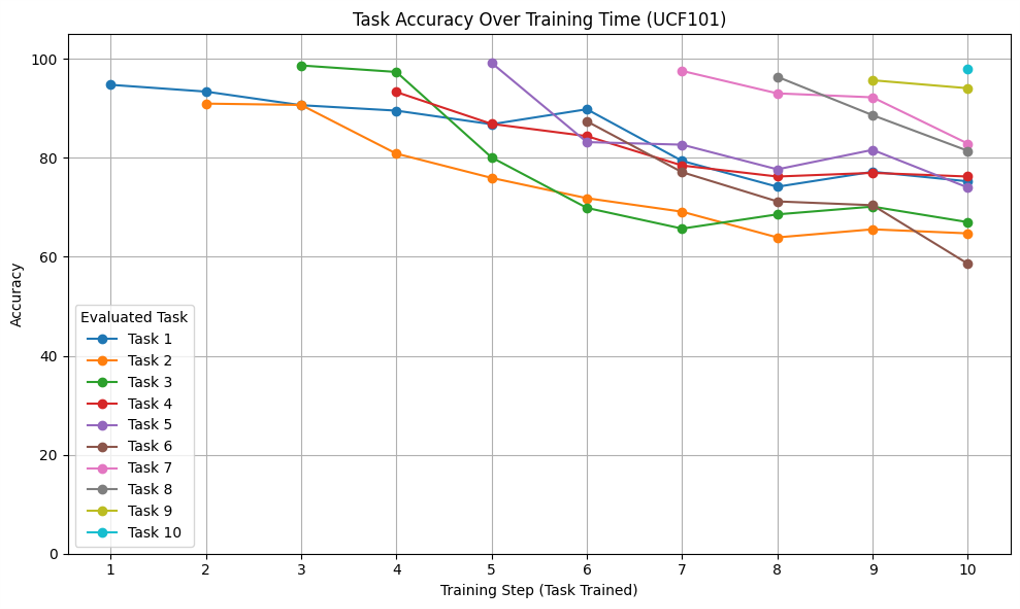
\includegraphics[width=0.45\textwidth]{Images/Chapter4/Random init fixed pool.png}
		\label{subfig:Random init fixed pool}
	}
	\caption[تغییرات صحت هر وظیفه در هر گام آموزشی در مجموعه‌داده‌ی
	\lr{UCF101} ]
	{
تغییرات صحت هر وظیفه در مراحل مختلف آموزش برای چهار پیکربندی متفاوت. صحت هر وظیفه به صورت جداگانه در هر نمودار، از زمان اضافه شدن آن به مدل، نشان داده شده است. در نمودار (الف) از مقداردهی اولیه با کدگذار \lr{CLIP} استفاده شده و هر دسته شامل ۵ پرامپت است و استخر پرامپت به صورت پویا به‌روزرسانی می‌شود. نمودار (ب) نیز از مقداردهی اولیه با کدگذار \lr{CLIP}  بهره می‌برد اما هر دسته ۲ پرامپت دارد و استخر پرامپت همچنان پویاست. در نمودار (ج) مقداردهی اولیه به صورت تصادفی انجام شده و به ازای هر دسته ۲ پرامپت به استخر پرامپت اضافه می‌شود. نمودار (د) نشان‌دهنده‌ی حالتی است که مقداردهی اولیه تصادفی بوده و از یک استخر پرامپت ثابت با اندازه ۱۰۲ استفاده شده است.
	}
	\label{fig:ablation_study_ucf101}
\end{figure}

\begin{figure}
	\centering
	\subfloat[استخر پویا\lr{CLIP init – 5/class – }]{
		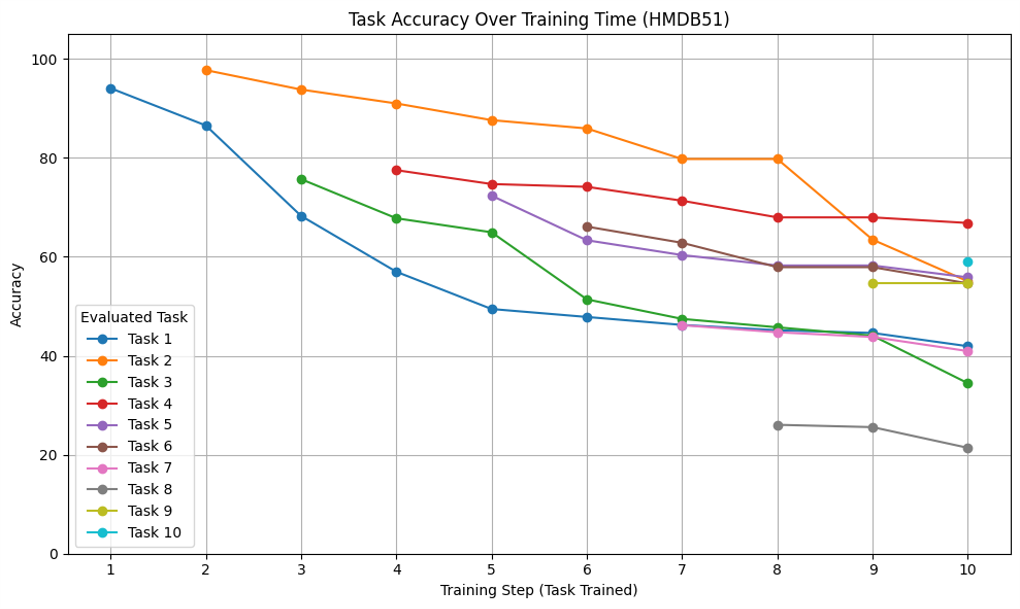
\includegraphics[width=0.45\textwidth]{Images/Chapter4/Encoder init 5 prompts class dynamic pool hmdb.png}
		\label{subfig:Encoder init 5 prompts class dynamic pool hmdb}
	}
	\quad
	\subfloat[استخر پویا\lr{CLIP init – 2/class – }]{
		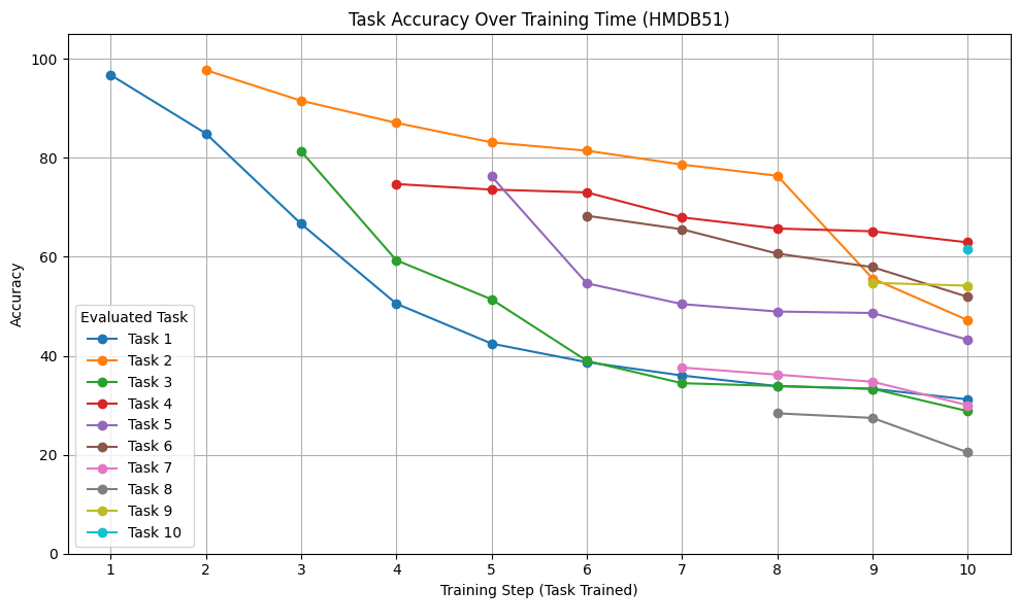
\includegraphics[width=0.45\textwidth]{Images/Chapter4/Encoder init 2 prompts class dynamic pool hmdb.png}
		\label{subfig:Encoder init 2 prompts class dynamic pool hmdb}
	}
	\caption[تغییرات صحت هر وظیفه در هر گام آموزشی در مجموعه‌داده‌ی
	\lr{HMDB51}]{
تغییرات صحت هر وظیفه در مراحل مختلف آموزش برای دو پیکربندی متفاوت. صحت هر وظیفه به صورت جداگانه در هر نمودار، از زمان اضافه شدن آن به مدل، نشان داده شده است. در نمودار (الف) از مقداردهی اولیه با کدگذار \lr{CLIP} استفاده شده و هر دسته شامل ۵ پرامپت است و استخر پرامپت به صورت پویا به‌روزرسانی می‌شود. نمودار (ب) نیز از مقداردهی اولیه با کدگذار \lr{CLIP} بهره می‌برد اما هر دسته ۲ پرامپت دارد و استخر پرامپت همچنان پویاست.
	}
	\label{fig:ablation_study_hmdb}
\end{figure}
\section{جمع‌بندی}
نتایج این فصل نشان می‌دهد که مدل \lr{ProActionCLIP} در یادگیری پیوسته‌ی تشخیص حرکت انسان، با دستیابی به میانگین صحت بالا، کاهش محسوس میزان فراموشی وظایف پیشین و بهره‌وری بالای محاسباتی، عملکردی برتری نسبت به روش‌های مرجع مانند \lr{PIVOT} دارد. همچنین آزمایش‌های تکمیلی نشان دادند که استفاده از مقداردهی اولیه با \lr{CLIP} و استخر پرامپت پویا، به‌ویژه با تعداد پرامپت‌های بیشتر، نقش مهمی در بهبود عملکرد مدل پیشنهادی ایفا می‌کند.



















